\chapter{Conexión y Compacidad}

\section{Conexión}
Una primera intuición nos puede decir que un conjunto es conexo si todos sus puntos están conectados. Por ejemplo el e.t. $(\bb{R}, \cc{T}_u)$ parece que es conexo mientras que otro espacio como el $([0,1]\cup\{2\}, \cc{T}_u)$ está hecho de varios ``trozos'' y por tanto no parece ser conexo. Incluso cambiando la topología puede ser que este segundo espacio fuese conexo (es por esto que no nos tenemos que dejar llevar siempre por la intuición).

\begin{definicion}
    Sea $(X, \cc{T})$ un e.t.
    \begin{itemize}
        \item Una \textbf{separación} de $(X, \cc{T})$ es una pareja de abiertos $\{U,V\}\subset \cc{T}$ que verifican $U\cup V = X$ y $U\cap V = \emptyset$.
        
        Se llama \textbf{separación trivial} a $\{X, \emptyset\}$.
        \item $(X, \cc{T})$ es \textbf{conexo} si su única separación es la trivial, es decir si $U,V\in \cc{T}$ con $U\cup V = X$ y $U\cap V = \emptyset$, entonces $U=\emptyset$ o $V=\emptyset$.
        \item $(X, \cc{T})$ es \textbf{disconexo} si no es conexo, es decir, si existen $U,V\in \cc{T}$ con $U\neq \emptyset$ y $V\neq \emptyset$ de forma que $U\cup V = X$ y $U\cap V = \emptyset$.
        \item Un subconjunto $A\subset X$ no vacío se dice \textbf{conexo} en $(X, \cc{T})$ si $(A, \cc{T}_A)$ es conexo y \textbf{disconexo} en caso contrario.
    \end{itemize}
    \endsquare
\end{definicion}

\begin{ejemplo}\
    \begin{itemize}
        \item $(X, \cc{T}_t)$ es conexo siempre.
        \item Si $\#X=1$ y consideramos $(X, \cc{T})$, entonces es conexo.
        \item Si $\#X\geq 2 \Rightarrow (X, \cc{T}_{disc})$ es disconexo. Para verlo podemos tomar $U\in \cc{T}_{disc}$ con $U\notin \{\emptyset, X\}$ y entonces tenemos $X\setminus U\in \cc{T}_{disc}$ y además $X\setminus U\neq \notin \{X, \emptyset\}$ y tenemos que $U\cap (X\setminus U) = \emptyset$ y $U\cup (X\setminus U) = X$.
        \item $(X, \cc{T}_{x_0})$ es conexo (si $U,V\in \cc{T}_{s_0}$ no vacíos, entonces $x\in (U\cap V) \neq \emptyset$).
        \item Si $\#=\infty \Rightarrow (X, \cc{T}_{CF})$ es conexo. Para verlo supongamos que existen $U,V\in \cc{T}_{CF}\setminus \{\emptyset\}$ con $U\cup V =X$ y $U\cap V = \emptyset$. Entonces $X\setminus U$, $X\setminus V$ son finitos y entonces $(U\setminus U)\cup (X\setminus V)$ es finito pero $(U\setminus U)\cup (X\setminus V) = X \setminus (U\cap V) = X$ que no es finito y por tanto llegamos a contradición.
        \item $(\{0,1\}, \cc{T}_u|_{[0,1]})$ es disconexo ya que $\{\{0\}, \{1\}\}$ es una separación.
        \item $(\{0,1\}, \cc{T})$ con $\cc{T}=\{\emptyset, \{0,1\}, \{0\}\}$ es conexo.
        \item $X=(\{0\}\times \bb{R})\cup (\{1\}\times \bb{R})\subset \bb{R}^2$ es disconexo en $\bb{R}^2$ en $(\bb{R}^2, \cc{T}_u)$.
        \item $[0,1]\cup \{2\}\subset \bb{R}$ es disconexo en $(\bb{R}, \cc{T}_u)$ 
        \item $\bb{Q}\subset \bb{R}$ es disconexo en $(\bb{R}, \cc{T}_u)$.
        \item $\bb{Z}$ es disconexo en $(\bb{R}, \cc{T}_u)$.
    \end{itemize}
    \endsquare
\end{ejemplo}

\begin{teo}
    Si $(X, \cc{T})$ es un e.t, entonces equivalem:
    \begin{enumerate}
        \item[(i)] $(X, \cc{T})$ es conexo.
        \item[(ii)] Si $A\in (\cc{T}\cap \cc{C}_{\cc{T}})$, entonces $A\in\{\emptyset, X\}$.
        \item[(iii)] $(X, \cc{T})$ cumple la \textbf{propiedad de los valores intermedios}\footnote{A partir de ahora lo notaremos por PVI}, es decir, si $f:(X, \cc{T})\to (\bb{R}, \cc{T}_u)$ continua y $a<b\in f(X)$, entonces $[a,b]\in f(X)$.
        \item[(iv)] Si $g:(X, \cc{T})\to (\{0,1\}, \cc{T}_{disc})$ es continua, entonces $g$ es constante 
    \end{enumerate}
    \begin{proof}\
        \begin{itemize}
            \item[(i)$\Rightarrow$(ii) )] $A\in \cc{T}\cap \cc{C}_{\cc{T}} \Rightarrow (X\setminus A) \in \cc{T} \Rightarrow \{A, X\setminus A\}$ es una separación de $(X, \cc{T})$. Por (i) tenemos que $\{A, X\setminus A\}=\{X, \emptyset\}$ por lo que $A\in \{\emptyset, X\}$.
            \item[(ii)$\Rightarrow$(iii) )] Sea $f:(X, \cc{T})\to (\bb{R}, \cc{T}_u)$ continua. Veamos que verifica la propiedad de los valores intermedios. Hagamos una distinción de casos:
            \begin{itemize}
                \item[$\bullet)$] Si $f$ es constante, entonces cumple trivialmente PVI.
                \item[$\bullet)$] Si $f$ no es constante podemos considerar $a<b\in f(X)$ y tendremos que ver que $[a,b]\subset f(X)$. Supongamos que no, es decir, que $\exists c\in (a,b)$ con $c\notin f(X)$. Definimos $A=f^{-1}((-\infty, c)) = f^{-1}((-\infty, c])$ y como $f$ es continua tenemos que $A\in (\cc{T}\cap \cc{C}_{\cc{T}})$ por lo que por (ii) sabemos que $A\in \{\emptyset, X\}$. Sin embargo, sabemos que $a\in f(X)$ y $a<c$ por lo que $A\neq \emptyset$. Además, $b\in f(X)$ pero $f^{-1}(b)\notin A$ por lo que $A\neq X$ y llegamos a contradicción.
            \end{itemize}
            \item[(iii)$\Rightarrow $(iv) )] Sea $g:(X, \cc{T}) \to (\{0,1\}, \cc{T}_{disc})$ continua. Sabemos que $\cc{T}_{disc}|_{\{0,1\}} = \cc{T}_u|_{\{0,1\}}$ y entonces podemos considerar la composición con la inclusión $i\circ g:(X, \cc{T})\to (\bb{R}, \cc{T}_u)$ es continua. Por (iii) sabemos que $(i\circ g)(X)\subset \bb{R}$ es un intervalo. Además, $(i\circ g)(X) = g(X)\subset \{0,1\}$ y es un intervalo (con la observación que viene a continuación). Esto implica que $g(X)=\{0\}$ o $g(X)=\{1\}$ lo cual implica que $g$ es constante.
            \item[(iv)$\Rightarrow$(i) )] Sea $\{U,V\}$ una separación de $(X, \cc{T})$. Veamos que $\{U,V\}=\{X, \emptyset\}$. Para ello considero la aplicación $g:(X, \cc{T})\to (\{0,1\}, \cc{T}_{disc})$ dada por 
            \begin{align*}
                g(x)=\left\{
                    \begin{array}{ccc}
                        0 & \text{ si } x\in U\\
                        1 & \text{ si } x \in V
                    \end{array}
                \right.
            \end{align*}
            Y tenemos que es continua ya que $g^{-1}(\{0\})=U\in \cc{T}$ y $g^{-1}(\{1\})=V\in \cc{T}$. Por (iv) tenemos que $g=cte$ y por tanto, $U =\emptyset$ o $V=\emptyset$ y como es una separación tenemos que $\{U,V\}=\{\emptyset, X\}$ y tenemos que $(X, \cc{T})$ es conexo.
        \end{itemize}
    \end{proof}
\end{teo}

\begin{observacion}
    A veces $[a,a]=\{a\}$ y lo llamaremos intervalo (a pesar de no ser estrictamente un intervalo según su definición formal). Con esto podríamos traducir el apartado (iii) del teorema anterior en que $f(X)$ sea un intervalo.
    \endsquare
\end{observacion}

\begin{coro}
    (Teorema de Bolzano)
    
    Si $(X, \cc{T})$ es conexo, $f:(X, \cc{T})\to (\bb{R}, \cc{T}_u)$ es continua y $\exists x,y\in X$ con $f(x)<0<f(y)$, entonces $\exists z \in X$ con $f(z)=0$. Esto es por cumplir la PVI.
    \endsquare
\end{coro}

\begin{coro}
    Si $(X, \cc{T})$ conexo y $f:(X, \cc{T})\to (\bb{R}, \cc{T}_u)$ continua con $f(x)\neq 0\ \ \forall x \in X$, entonces $f>0$ o $f<0$ en todo $X$.
    \endsquare
\end{coro}

\begin{coro}
    Si $\emptyset\neq A \subset \bb{R}$, entonces $A$ es conexo en $(\bb{R}, \cc{T}_u)\sii A$ es unitario o $A$ es un intervalo.

    \begin{proof}\
        \begin{itemize}
            \item[$\Leftarrow$)] Si $A$ es unitario es conexo. Si $A$ es un intervalo, entonces $(A, \cc{T}_u|_A)$ cumple la PVI\footnote{la estudiada en la asignatura de Cálculo I} y por el teorema tenemos que $A$ es conexo en $(\bb{R}, \cc{T}_u)$.
            \item[$\Rightarrow$)] Supongamos que $A$ es conexo y que no es ni unitario ni un intervalo. Por tanto existen $a<c<b$ tales que $a,b\in A$ pero $c\notin A$. Consideramos $U=(-\infty, c)\cap A$, $V=(c, +\infty)\cap A$ y tenemos que $\{U,V\}$ es una separación de $(A, \cc{T}_u|_A)$ que no es trivial ya que $a\in U$ y $b\in V$ por lo que $(A, \cc{T}_u|_A)$ es disconexo y llegamos a contradicción.
        \end{itemize}
    \end{proof}
\end{coro}

\begin{observacion}
    La conexión no es una propiedad hereditaria.
    \endsquare
\end{observacion}

\begin{coro}
    Si $(X, \cc{T})$ es conexo y $f:(X, \cc{T})\to (Y, \cc{T}')$ es continua, entonces $f(X)$ es conexo en $(Y, \cc{T}')$. \\
    
    Si $f$ es además sobreyectiva, entonces $(Y, \cc{T}')$ es conexo.
    \begin{proof}
        Tenemos que comprobar que $(f(X), \cc{T}'|_{f(X)})$ es conexo. Para ello consideramos $g:(f(X), \cc{T}'|_{f(X)})\to (\{0,1\}, \cc{T}_{disc})$ continua y tendremos que ver que $g=cte$. Tomamos $g\circ f^{f(X)}:(X, \cc{T})\to (\{0,1\}, \cc{T}_{disc})$ que es continua (por ser composición de continuas) y además, por hipótesis tenemos que $(X, \cc{T})$ es conexo por lo que $g\circ f^{f(X)}$ es constante y por tanto $g$ es constante y por el teorema anterior tenemos lo buscado.
    \end{proof}
\end{coro}

\begin{coro}
    \begin{enumerate}
        \item[(i)] La conexión es un invariante topológico.
        \item[(ii)] Si $f:(X, \cc{T})\to (Y, \cc{T}')$ es una identificación y $(X, \cc{T})$ es conexo, entonces $(Y, \cc{T}')$ es conexo.
        \item[(iii)] Si $(X, \cc{T})$ es conexo y $R$ es una relación de equivalencia en $X$, entonces $(X/R, \cc{T}/R)$ es conexo.
        \item[(iv)] $(\bb{S}^1, \cc{T}_u|_{\bb{S}^1})$ es conexo.
        \item[(v)] $[a,b], [a,b), (a,b]$ y $(a,b)$ no son homeomorfos en $(\bb{R}, \cc{T}_u)$ 
        \item[(vi)] $(\bb{R}\setminus \{x\}, \cc{T}_u)$ no es homeomorfo a $(\bb{R}, \cc{T}_u)$.
        \item[(vi)] $(\bb{R}, \cc{T}_u)$ no es homeomorfo a $(\bb{S}^1, \cc{T}_u|_{\bb{S}^1})$.  
    \end{enumerate}
    \begin{proof}\
        \begin{enumerate}
            \item[(i),(ii),(iii)] Triviales.
            \item[(iv)] Sabemos que $([0,1], \cc{T}_u|_{[0,1]})$ es conexo y tenemos que existe una función $f:([0,1], \cc{T}_u|_{[0,1]})\to (\bb{S}^1, \cc{T}_u)$ es continua y sobreyectiva, por ejemplo, $f(t)=(\cos(2\pi t), \sen(2\pi t))$.
            \item[(v)] Supongamos que $[a,b)\cong(a,b)$. Entonces tenemos que existe un homeomorfismo $f:([a,b), \cc{T}_u)\to ((a,b), \cc{T}_u)$. Pero entonces $f|_{[a,b]}:([a,b), \cc{T}_u)\to ((a,b)\setminus \{f(a)\}, \cc{T}_u)$ sería un homeomorfismo pero llegaríamos a contradicción ya que la conexión es un invariante topológico.
            \item[(vi),(vii)] Se dejan planteadas como ejercicios para el lector.  
        \end{enumerate}
    \end{proof}
\end{coro}

\begin{teo}
    (Teorema del punto fijo) Si $f:([0,1], \cc{T}_u)\to ([0,1], \cc{T}_u)$ continua, entonces $\exists x_0 \in [0,1]$ con $f(x_0)=x_0$.
    \begin{proof}
        Sea $h:[0,1]\to [0,1]$ con $h(x)=f(x)-x$ continua. Tenemos que $[0,1]$ es conexo luego
        \begin{align*}
            \left.
            \begin{array}{c}
                h(0)=f(0)\geq 0\\
                h(1)=f(1)-1 \leq 0\\
            \end{array}
            \right\} &\overset{PVI}{\Rightarrow} 0 \in [h(1),h(0)] \subset h([0,1]) \Rightarrow \exists x_0 : h(x_0)=0 \Rightarrow \\
            &\Rightarrow f(x_0) = x_0
        \end{align*}
    \end{proof}
\end{teo}

\begin{teo}
    (Teorema de la invariaza del dominio) Si $A\neq \emptyset $ es abierto en $(\bb{R}, \cc{T}_u)$ y $f:(A, \cc{T}|_A)\to (\bb{R}, \cc{T}_u)$ es un embebimiento, entonces $f(A)$ es abierto en $(\bb{R}, \cc{T}_u)$.

    \begin{proof}
        Sabemos que $A\in \cc{T}_u$ y además $A\neq \emptyset$ luego podemos escribir $A=\bigcup\limits_{i\in I}I_i$ donde $I_i$ es un itervalo abierto en $(\bb{R}, \cc{T}_u)$\ \ $\forall i \in I$, luego tenemos que $f(A)=f(\bigcup\limits_{i\in I})=\bigcup\limits_{i\in I}f(I_i)$. Si conseguimos ver que $f(I_i)\in \cc{T}_u\ \ \forall i \in I$ tendremos lo buscado. 

        Sabemos que $I_i$ es conexo y $f$ es continua luego $f(I_i)$ es conexo en $(\bb{R}, \cc{T}_u)$ y por tanto es un intervalo (no unitario porque $f$ es inyectiva). Además, como $f$ es un embebimiento tenemos que $f(I_i)\cong I_i$ que es un intervalo abierto por lo que $f(I_i)$ será también un intervalo abierto y entonces $f(I_i)\in \cc{T}_u$. Como $i$ era arbitrario tenemos lo buscado.

    \end{proof}
\end{teo}

 \section{Construcción de conexos}

 En general, la unión de conexos no es conexo. En $(\bb{R}, \cc{T}_u)$ tenemos que $]0,1[\cup]2,3[$ no es conexo. La intersección tampoco lo será. Por ejemplo, en $(\bb{S}^1, \cc{T}_u)$ podemos imaginar 2 abiertos que se ``crucen'' y su intersección no será conexa (ya que generará otros 2 abiertos que no estarán conectados) como se ve en la figura a continuación:
\vspace*{0.25cm}
\begin{center}
    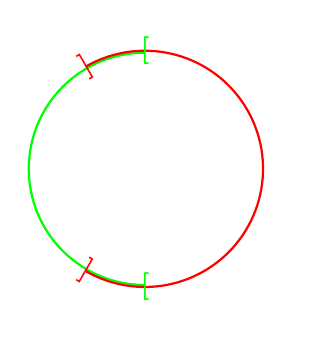
\begin{tikzpicture}
        % Dinujar la mitad verde
        \draw[green, thick] (90:1.475cm) arc[start angle=90, end angle=270, radius=1.475cm];
        % Dibujar la mitad roja
        \draw[red, thick] (120:1.5cm) arc[start angle=120, end angle=-120, radius=1.5cm];
        
        \node[color=red, rotate=30] at (120:1.5cm) {\textbf{]}};
        \node[color=red, rotate=-30] at (-120:1.5cm) {\textbf{]}};

        \node[color=green] at (90:1.5cm) {\textbf{[}};
        \node[color=green] at (-90:1.5cm) {\textbf{[}};
     \end{tikzpicture}
\end{center}

\begin{prop}
    Sea $(X, \cc{T})$ un e.t., $\{A_i\}_{i\in I}$ una familia de conexos en $(X, \cc{T})$. Se tienen:
    \begin{enumerate}
        \item[(i)] Si $\exists i_o \in I$ tal que $A_i\cap A_{i_0}\neq \emptyset \ \ \forall i\in I$, entonces se tiene que $\bigcup\limits_{i\in I}A_i$ es conexo en $(X, \cc{T})$.
        \item[(ii)] Si $\bigcap\limits_{i\in I} A_i \neq \emptyset \Rightarrow \bigcup_{i\in I} A_i$ es conexo en $(X, \cc{T})$.
        \item[(iii)] Si $I=\bb{N}$ y $A_n\cap A_{n+1}\neq \emptyset$\ \ $\forall n\in \bb{N}$, entonces $\bigcup\limits_{n\in \bb{N}}A_n$ es conexo en $(X, \cc{T})$.  
    \end{enumerate}
    \begin{proof}\
        \begin{enumerate}
            \item[(i)] Sea $g:(\bigcup\limits_{i\in I}A, \cc{T}_u)\to (\{0,1\}, \cc{T}_{disc})$ continua. Entonces $\forall i \in I$ consideramos $g|_{A_i}:(A_i, \cc{T}_u)\to (\{0,1\}, \cc{T}_{disc})$ continua. Entonces tenemos que $g|_{A_i}$ es constante. En particular, $g|_{A_{i_0}}=c_{i_0}$. Tendremos que ver que $c_i=c_{i_0}$\ \ $\forall i \in I$. 
            Como $A_i\cap A_{i_0}\neq \emptyset$, entonces $\exists x \in A_i \cap A_{i_0}$ y entonces
            \begin{align*}
                \left. 
                \begin{array}{c}
                    c_i=g|_{A_i}(x) = g(x)\\
                    c_{i_0}=g|_{A_{i_0}}(x) = g(x)\\
                \end{array}
                \right\} \Rightarrow c_{i_0}=c_i \Rightarrow g \text{ es constante }\Rightarrow \bigcup\limits_{i\in I}A_i \text{ conexo}
            \end{align*}
            \item[(ii)] Corolario de (i).
            \item[(iii)] Se deja planteado como ejercicio para el lector.
        \end{enumerate}
    \end{proof}
\end{prop}

\begin{ejemplo}\
    \begin{itemize}
        \item $A\subset \bb{R}^n$ se dice \textbf{estrellado} si $\exists x_0 \in A$ tal que $[x,x_0]^n = \{(\lambda x_0 + (1-\lambda)x):\lambda \in [0,1]\}\subset A\ \ \forall x \in A$, es decir, si el segmento que une cualquier punto $x$ de $A$ con el punto $x_0$ está contenido en $A$.
        
        En $(\bb{R}, \cc{T}_u)$ todo subconjunto estrellado es conexo, $A=\bigcup\limits_{x\in A}[x,x_0]$, con $x_0\in \bigcap\limits_{x\in A}[x,x_0]\neq \emptyset$ y $[x,x_0]$ es conexo. En particular, todo subespacio afín de $\bb{R}^n$, las bolas abiertas y cerradas y los convexos de $\bb{R}^n$ son conexos.

        \item $(\bb{S}^n, \cc{T}_u)$ es conexo. Para verlo, podemos considerar $\bb{S}^n=(\bb{S}^n\setminus \{N\})\cup (\bb{S}^n \setminus \{S\})$ y como $(\bb{S}^n\setminus \{N\}) \cong \bb{R}^n \cong(\bb{S}^n\setminus \{S\})$ entonces $\bb{S}^n$ es unión de conexos con intersección no vacía.
        
        \item Si $n\geq 2$, entonces $\bb{R}^n \setminus\{0\}$ es conexo, ya que $\bb{R}^{n+1} \setminus \{0\}=\bigcup\limits_{x\in \bb{R}^{n+1}\setminus \{0\}} \left(\bb{S}^n\cup \left[x, \frac{x}{\|x\|}\right] \right)$. Además, como $\bb{R}^n\setminus\{x\}\cong \bb{R}^n \setminus\{0\}$ (aplicando una traslación $y\mapsto y-x$), entonces también será convexo $\forall x \in \bb{R}^n$.
    \end{itemize}
    \endsquare
\end{ejemplo}

\begin{coro}\
    \begin{enumerate}
        \item[(i)] $\bb{R}\ncong \bb{R}^n$\ \ $\forall n\geq 2$ ya que $\bb{R}^n\setminus\{x\}$ es conexo pero $\bb{R}\setminus \{0\}$ no lo es.
        \item[(ii)] $\bb{S}^1 \ncong \bb{S}^n$\ \ $\forall n \geq 2$ porque $\bb{S}^1\setminus \{x\}\ncong \bb{S}^n\setminus \{x\}$ ya que $\bb{S}^1\setminus \{x\}\cong \bb{R} \ncong \bb{R}^n \cong \bb{S}^n \setminus \{x\}$. 
    \end{enumerate}
    \endsquare
\end{coro}

\begin{teo}
    (Teorema de Borsuk-Ulam) Si $f:(\bb{S}^n, \cc{T}_u)\to (\bb{R}, \cc{T}_u)$ continua, entonces $\exists p_0\in \bb{S}^n$ tal que $f(p_0)=p(-p_0)$.
    \begin{proof}
        Sea $h:\bb{S}^n \to \bb{R}$ dada por $h(p)=f(p)-f(-p)$ que es continua por serlo $f$. Se tiene que $h(-p)=f(-p)-f(p)=-h(p) \Rightarrow h\equiv 0$ o $h$ toma valores negativos y negativos. En este segundo caso tendremos que $\exists p_0 \in \bb{S}^n$ tal que $h(p_0)=0=f(p_0)-f(-p_0)$ y lo tenemos en cualquiera de los dos casos.

    \end{proof} 
\end{teo}

\begin{prop}
    Sea $(X, \cc{T})$ un e.t. y $A\subset X$ conexo. Si $B\subset X$ cumple $A\subset B \subset \overline{A}$, entonces $B$ es conexo. En particular, $\overline{A}$ es conexo.
    \begin{proof}
        Sea $f:(B, \cc{T}_B)\to (\{0,1\}, \cc{T}_{disc})$ continua. Tendremos que ver que $f$ es constante. Para ello, como $A\subset B$, puedo tomar $\overline{A}^B=\overline{A}\cap B = B$ por lo que $A$ es denso en $B$. Por otra parte, $f(\overline{A}^B)\subset \overline{f(A)}$, y como $A$ es conexo, $f|_A$ es continua y constante $\Rightarrow f(A)=\{0\}$ o $f(A)=\{1\}$. En cualquier caso tendremos $\overline{f(A)}=\{0\}$ o $\overline{f(A)}=\{1\}$, luego $f$ es constante porque $f(B)\subset f(A)$.

    \end{proof}
\end{prop}

\begin{ejemplo}\
    \begin{itemize}
        \item Sea $(X, \cc{T})$ un e.t. y supongamos que existe $A\subset X$ denso y conexo, entonces $(X, \cc{T})$ es conexo.
        \item $f:]0,1] \to \bb{R}$, $x\mapsto \sen\left(\frac{1}{x}\right)$, $A=G(f)=\left\{\left(x, \sen\left(\frac{1}{x}\right)\right): x\in ]0,1]\right\}$. Entonces $A\cong ]0,1]$ que es conexo. Esto quiere decir que la gráfica de una función es homeomorfa al dominio de la aplicación,
        \begin{align*}
            A & \to ]0,1]\\
            \left(x, \sen\left(\nicefrac{1}{x}\right)\right) & \mapsto x
        \end{align*}
        Además, $\overline{A}=A\cup[(0,1),(0,-1)]$ es conexo.
    \end{itemize}
    \endsquare
\end{ejemplo}

\begin{prop}
    Sean $(X, \cc{T})$, $(Y, \cc{T}')$ e.t. Entonces $(X\times Y, \cc{T}\times \cc{T}')$ es conexo si y solo si $(X, \cc{T})$ y $(Y, \cc{T}')$ son conexos.
    \begin{proof}\
        \begin{itemize}
            \item[$\Rightarrow$)] Como las proyecciones $\pi_X$ y $\pi_Y$ son continuas y sobreyectivas, esta implicación es trivial.
            \item[$\Leftarrow$)] Sabemos que $(X, \cc{T})$ es conexo. Sea $y\in Y$ tenemos que $(X\times \{y\}, \cc{T}\times \cc{T}'|_{X\times\{y\}})\cong (X, \cc{T})$ que es conexo. Si consideramos ahora $x\in X$ y  $(\{x\}\times Y, \cc{T}\times \cc{T}'|_{\{x\}\times Y})\cong (Y, \cc{T}')$. Con esto tenemos que
            \begin{align*}
                X\times Y = \left(\bigcup\limits_{x\in X}\{x\}\times Y\right) \cup \left(X \times \{y_0\}\right)
            \end{align*}
            Por lo que $X\times Y$ es unión de conexos y $(X, \{y_0\})$ tiene intersección con todos los $\{x\}\times Y$ luego $X\times Y$ es conexo.

        \end{itemize}
    \end{proof}
\end{prop}

\begin{ejemplo}
    Los siguientes conjuntos son conexos:
    \begin{itemize}
        \item $\bb{S}^1 \times \bb{R}$ (cilindro).
        \item $\bb{T}=\bb{S}^1 \times \bb{S}^1$ (toro).
        \item $\bb{R}\bb{P}^n = \bb{R}^{n+1}\setminus \{0\}/R$ (proyectivo).
        \item La cinta de Möbius.
    \end{itemize}
    \endsquare
\end{ejemplo}
